\documentclass{article}
\usepackage[margin=2.5cm]{geometry}
\usepackage{enumerate, fancyhdr, graphicx, amsmath}

\def\tetris{Tetris\textsuperscript{\textregistered}}

\title{Old School \tetris{} Meets Game Tree Search}
\author{Paul Chesnais (pmc85) and Sam Svenningsen (sjs382)}
\date{\today}

\pagestyle{fancy}
\fancyhead{}
\lhead{pmc85 and sjs382}
\chead{PRAC CS 4700 - Proposal}
\rhead{\today}
\fancyfoot{}
\rfoot{\thepage}
\lfoot{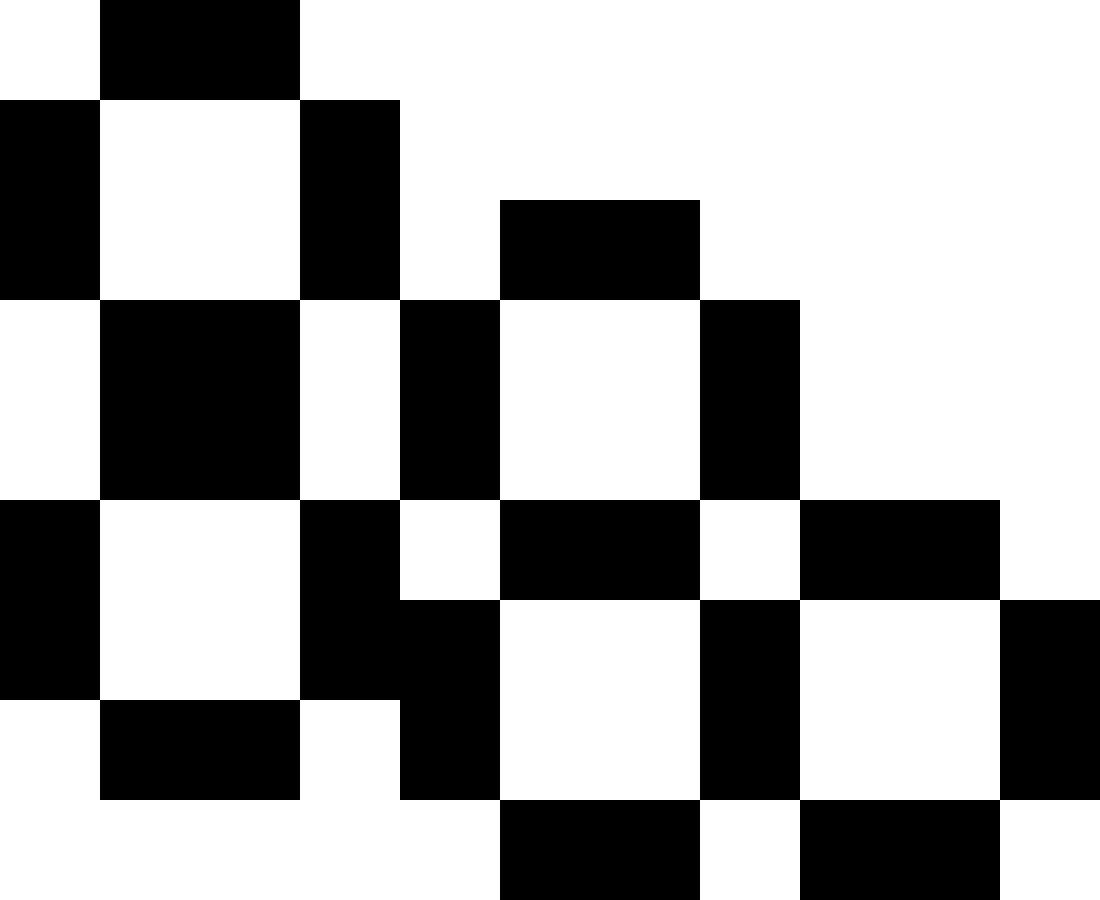
\includegraphics[height=20pt]{Logo}}
\renewcommand{\headrulewidth}{0.5pt}
\renewcommand{\footrulewidth}{0.5pt}

\newcommand{\exo}[1]{\section*{Exercise #1}}
\newcommand{\prob}[1]{\section*{Problem #1}}
\newcommand{\quest}[1]{\section*{Question #1}}
\newcommand{\e}{&=&}
\newcommand{\p}[1]{\times 10^{#1}}

\begin{document}
\maketitle
\thispagestyle{empty}

\section{Description}

\par For our Project in the AI Practicum, we plan on building a \tetris{} bot. Ideally, this bot would play at speeds far greater than normal human speed, and if at all possible, when faced with the original implementation of \tetris{}, would beat the current human world record. We believe that such a task would be quite interesting to attack, and if done well, could in fact teach us a lot about what it is like to play a ``perfect'' \tetris{} game, or what strategies seem to work better than most.

\section{Possible approaches}

\par There are multiple ways to approach solving, or playing, \tetris{}. For shorthand, we will refer to the current state of the game or the ``board'', i.e. all the stacked pieces, as the stack.

\paragraph{Iterative Tree} An obvious choice would be to, given a particular piece, attempt to place in every rotation and every position, and according to some cost metric, pick the least expensive or most likely to create a good board for the next piece. If we have a lookahead, i.e. we know what piece is coming next, like in most popular \tetris{} games, we can even try all the combinations of each piece and pick which is best. Unfortunately, this method might actually take a while to compute, and may not finish computing until the piece drops and we lose control of it.
\paragraph{Ranking} There is another method in which we look at the game completely differently. Suppose we want to enforce a guarantee that at all times, none of the pieces we have placed have created a hole in the stack. In other words, no hole is created that cannot be filled immediately with the right piece. If this is the case then the only thing we need to look at is the shape of the top layer, let's call it the contour. Suppose we managed to rank every single contour, then all we need to do is pick the position of the falling piece that creates the best ranking contour.

\section{Plan}

Try different approaches to compare success and easiness. Success being average score and max highest score with each approach.

\begin{description}

  \item[Graph Traversal (Look for actual name)] Calculate all possibilities n moves ahead, choose best. Best being a ``perfect'' Tetris stack (i.e. no holes) for as many consecutive pieces as possible.

  \item[Heuristic Approach] Find out if we can get a heuristic function that gives a score to a tetris state plus a new piece or pieces in any configuration and choose the max (or min) value one.

  \item[A* search]

  \item[Reinforcement Learning]?

\end{description}


\section{Timeline}



\end{document}
